\begin{frame}
  \frametitle{Sistemas de diálogo Humano-Computadora}

  \begin{enumerate}[<+->]
    \item Sistemas actuales
    \item Bien en la parte lingüística de la comunicación: entender y transmitir mensajes estructuralmente correctos.
    \item Mal en la parte superestructural: intercambio de emociones, actitudes, etc.
    \item El presente trabajo trata de hacer un (pequeño) aporte sobre el análisis de la ``naturalidad'' de las conversaciones.
  \end{enumerate}
\end{frame}


\begin{frame}
  \begin{columns}
    \column{0.5\textwidth}
    \frametitle{Ejemplos de ``falta de naturalidad''}
    \begin{enumerate}
      \item Sistemas de llamadas comerciales
      \item Siri, Google Now
      \item Otros?
    \end{enumerate}
    \column{0.5\textwidth}
    \begin{figure}
      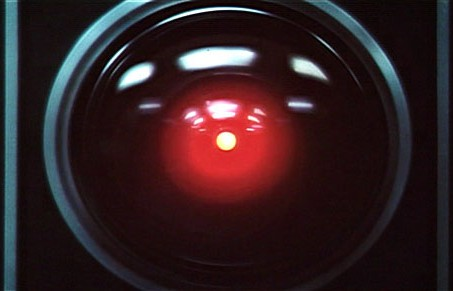
\includegraphics[scale=0.25]{images/hal.jpg}
    \end{figure}
  \end{columns}
\end{frame}


\begin{frame}
  \frametitle{Prosodia}
  \framesubtitle{Definir acá qué es la prosodia aproximadamente}

\end{frame}



\begin{frame}
  \frametitle{Entrainment}

  \begin{enumerate}
    \item Fenómeno ubícuo en la comunicación
    \item Ocurre a varios niveles
    \item Largamente estudiado en psicología de comportamiento (referencias)
    \item (ya está, la próxima conversación que tengan afuera de acá van a chequear ésto)
  \end{enumerate}
\end{frame}

\begin{frame}
  \frametitle{¿Y cómo lo medimos?}
  La definición de entrainment hasta acá vista es heurística! ¿Cómo definimos una medida para esto?

  Vamos a explorar una métrica definida en trabajos anteriores, pulirla un poco, y verificar que efectivamente capture ciertas características del entrainment.

  ¿Cómo? Usando un corpus con anotaciones sociales


\end{frame}
